\section{Optimization}
In the following, we present high-level methods that we used to gradually
improve the performance of the algorithm. We name the different implementations
that we obtained according to the methods we employed. The following graph gives
an overview over the development of the different versions:

\begin{figure}[htb]
\centering
% \includegraphics[width=10cm]{AdvCompSetup}
\caption{An example of a figure.}
\label{fig:AdvCompSetup}
\end{figure}

\begin{figure}

\begin{center}
\begin{tikzpicture}[-,shorten >=1pt,auto,node distance=1.8cm,
  thick,main node/.style={font=\sffamily\scriptsize\bfseries}]
	
  \node[main node] (1) {Transposed};
	\node[main node] (2) [below=1em of 1] {Bottom-Up};
	\node[main node] (3) [below=1em of 2] {Partial-Results};
	\node[main node] (4) [below left=1em and 1em of 3] {Triangular};
	\node[main node] (5) [below=1em of 4] {Vectorized, Triangular};
	\node[main node] (6) [below right=1em and 1em of 3] {Blocking};
	\node[main node] (7) [below=1em of 6] {Vectorized, Blocking};

  \path[every node/.style={font=\sffamily\small}]
	(1) edge node [below] {} (2)
		(2) edge node [below] {}(3)
		(3) edge node [below] {}(4)
		(4) edge node [below] {}(5)
		(3) edge node [below] {}(6)
		(6) edge node [below] {}(7)
		;
\end{tikzpicture}
\label{fig:DecTree}
\end{center}
\caption{Overview of optimizations.}
\end{figure}

\begin{figure}[htb]\centering
	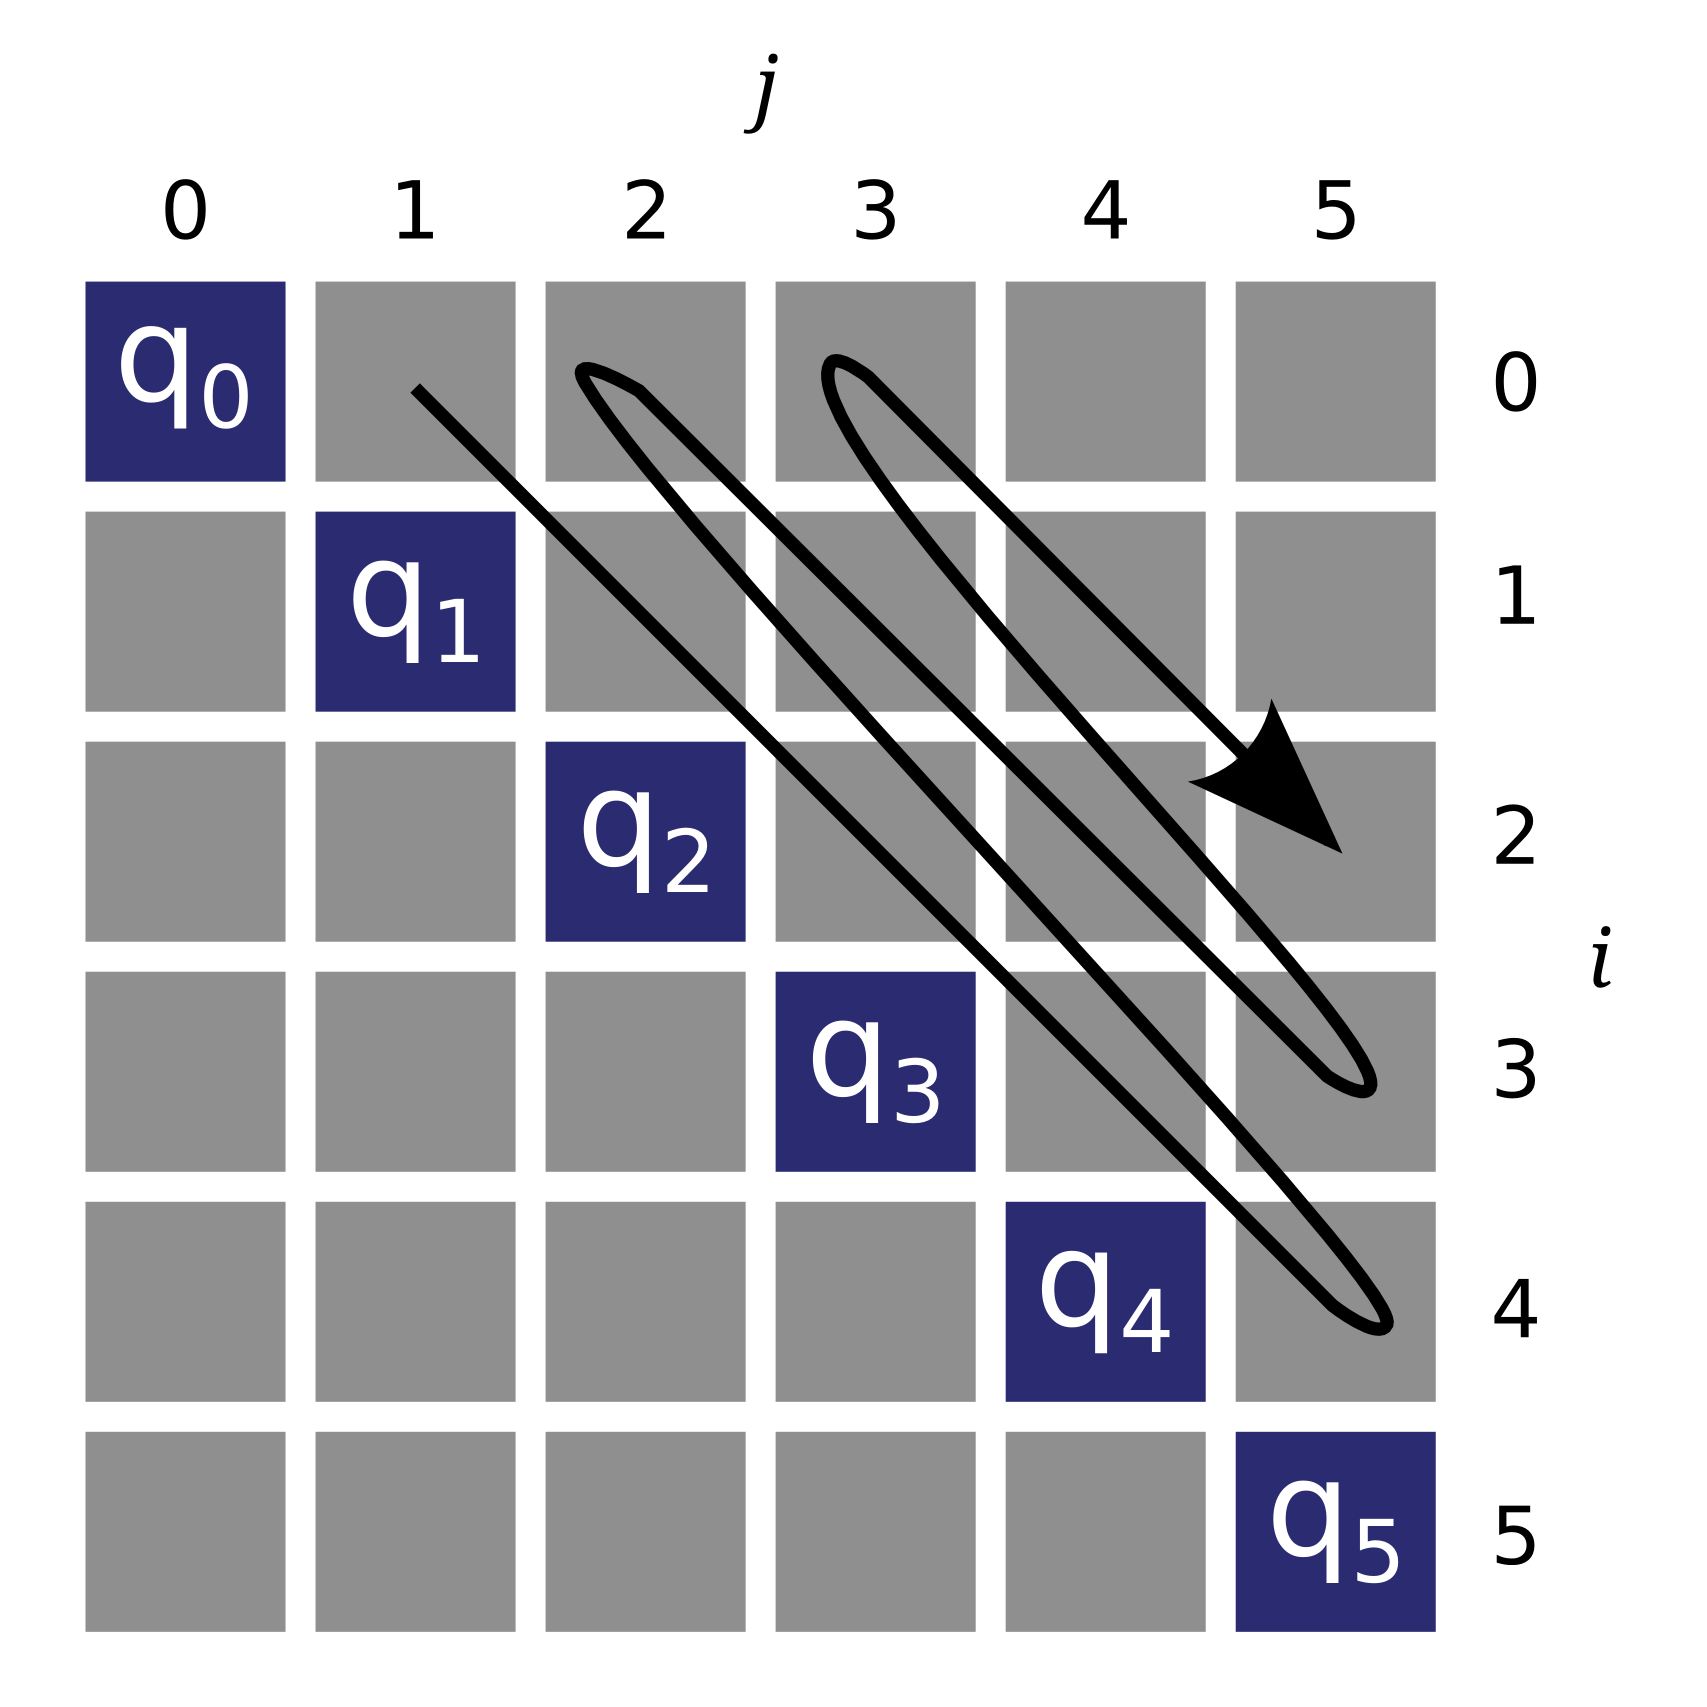
\includegraphics[width=0.33\textwidth]{img/reference_access.png}
  \caption{Access Pattern of reference implementation.\label{fig:reference}}
\end{figure}

\mypar{Transposed} Examining the innermost loop, we see that the table is
accessed row- and column-wise. Thus, the memory is accessed in strides of $1$
and $n+1$, respectively. However, with two simple changes to the algorithm, we
can avoid strides of $n+1$ and replace them with accesses of stride $1$: We make
use of the lower half of the square table in that we store newly calculated
values not only at $(i,j)$ but also at $(j,i)$. That is, instead of accessing a
column in the upper half, we access a row in the lower-half. This needs only two
minor changes to the algorithm as described in listing \ref{lst:baseline}:
First, line $7$ turns into
\begin{center}
\verb:t = e[IDX(i,r)] + e[IDX(j,r+1)]:, 
\end{center}
and after line $10$, we would insert 
\begin{center}
	\verb:e[IDX(j,i)] = t;:.
\end{center}
\mypar{Bottom-Up} The order in which individual values are calculated is along
the diagonals, as visualized in Figure \ref{fig:reference}. We notice that, for
two distinct cells on a diagonal, their corresponding rows and columns intersect
exactly in one cell. By changing the outermost two loops such that the table is
being built up row-wise and bottom-up (as visualized in Figure
\ref{fig:bottom-up}) we can thus
improve the temporal locality with respect to the accesses to the row that is
currently being built-up.

\begin{figure}[htb]\centering
	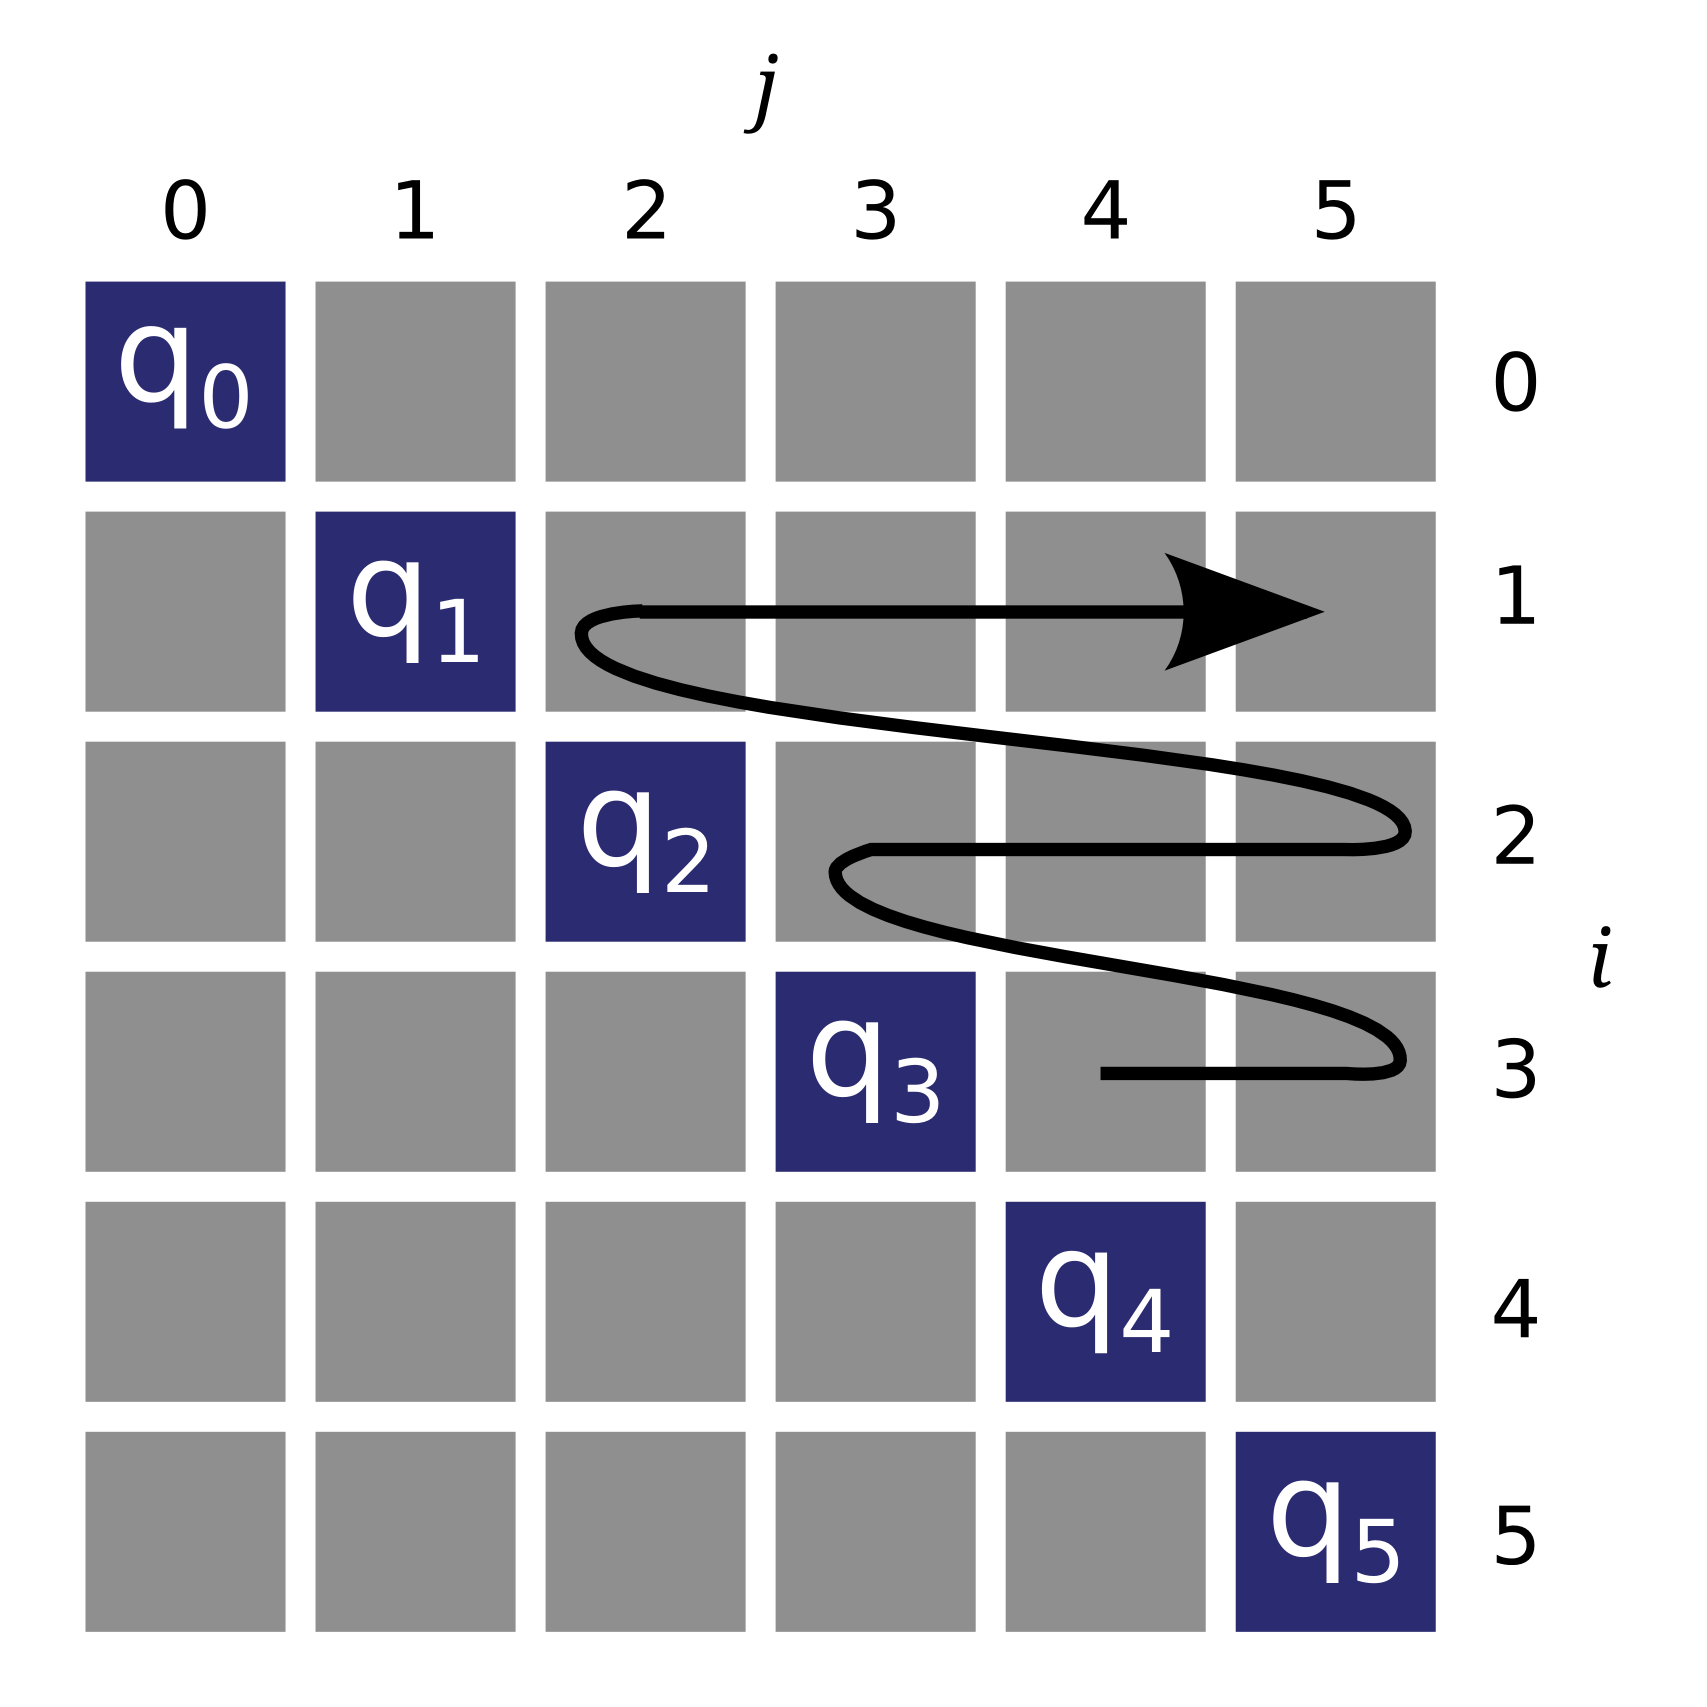
\includegraphics[width=0.33\textwidth]{img/bottom_up_access.png}
  \caption{Access Pattern of Bottom-Up.\label{fig:bottom-up}}
\end{figure}

\mypar{Partial Results} Instead of calculating the minimum value over a full row
and column, we can store intermediate values for an entire row by swapping the
innermost two loops. That is, for row $i$, we add the value $e[i,r], i\leq r\leq
n$ to all entries $e[r,j], r\leq j \leq n$ and store the minimum of that sum and
$e[i,r]$ in $e[i,r]$. Figure visualize the pattern for one
consecutive executions of the $r$-loop (which is now the second innermost loop):
the value contained in the cell with the unfilled circle is added to all values
contained in the cells with the filled circle and the minimum is stored in the
cells that are empty.

\begin{figure}[htb]\centering
	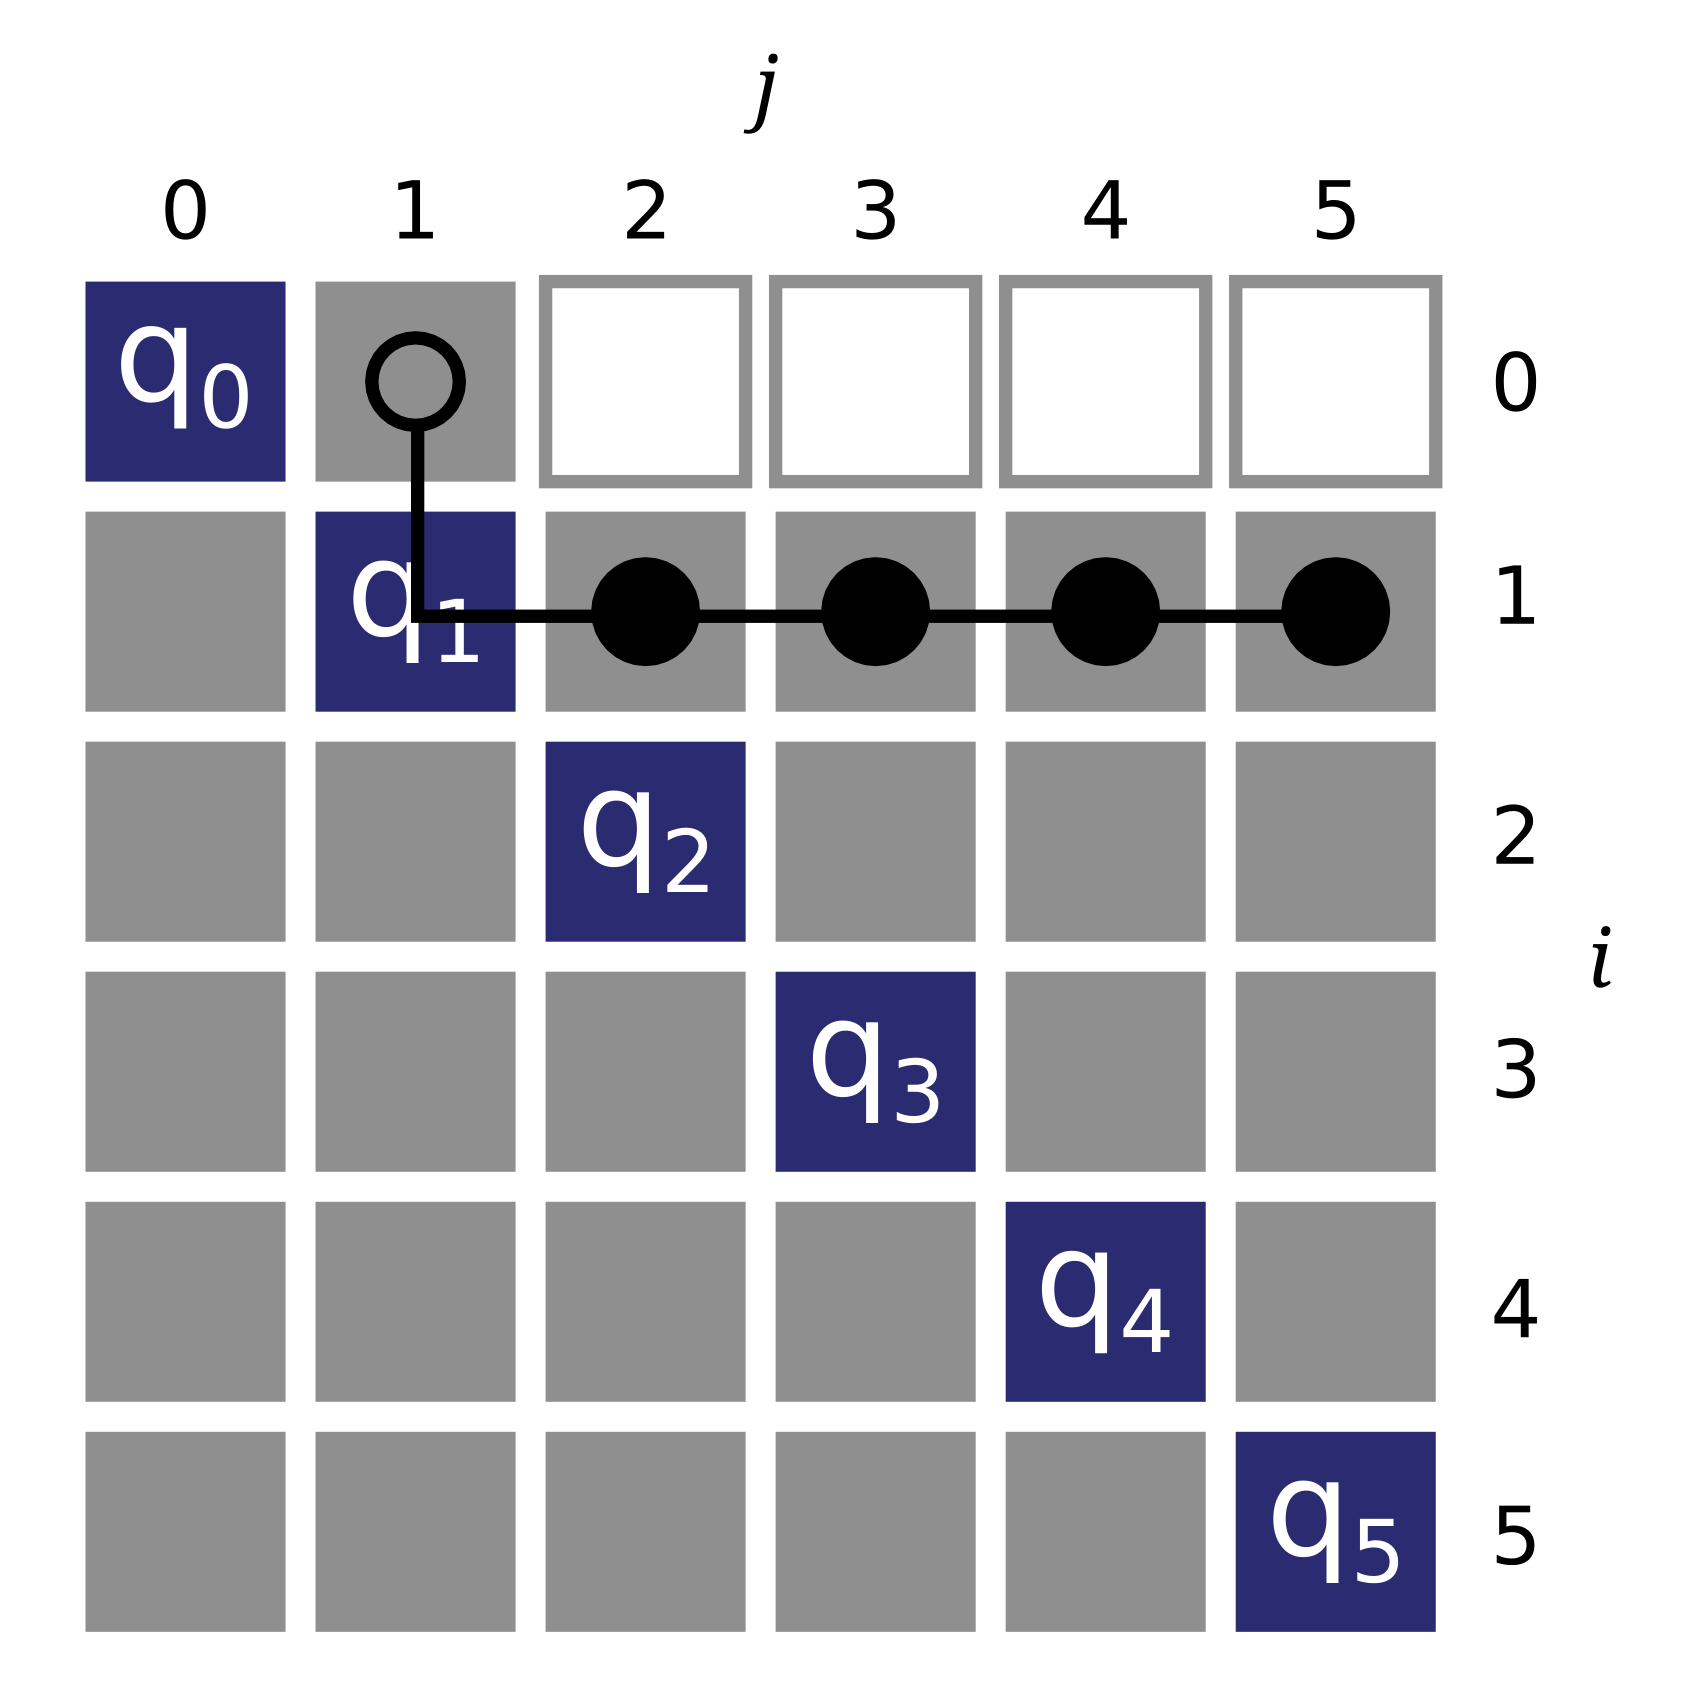
\includegraphics[width=0.33\textwidth]{img/intermediate_access.png}
  \caption{Storing Partial results.\label{fig:partial}}
\end{figure}

\mypar{Triangular} While the above approach itself does not improve the
performance over the \emph{Bottom Up}-approach, we notice that employing this
pattern, we can omit mirroring the table and still all but the first memory
access in the innermost loop have stride $1$. Hence, we can \emph{compress} the
memory layout by just concatenating the rows of the ``upper'' triangular table.
We call this memory layout \emph{triangular}--as opposed to the \emph{square}
layout.

Experimental results show that this indeed increases the performance. We assume
that this is due to the hardware prefetcher not loading unused parts of the
table into cache, but we lack the necessary hardware equipment to verify this
assumption.

On the downside, using this memory layout significantly complicates the
calculation of indices. For instance, the correct index-macro for this memory
layout is defined as follows:
\begin{center}
	\scriptsize
	\begin{verbatim}#define IDX(i,j)\
	((n+1)*(n+2)/2 - (n-(i)+1)*(n-(i)+2)/2 + (j) - (i))\end{verbatim}
\end{center}
This problem can be alleviated by doing strength reduction. That is, we
introduce separate index variables which hold the indices for the values being
calculated and being read independently from the loop variables. In most cases,
additions and subtractions are sufficient to update these variables.

\mypar{Vectorized Triangular} Historically, our initial approaches at
blocking (our final blocking approach is explained below) were unsuccessful.
Thus, we focused on vectorizing the Triangular Layout, which is
straight-forward: The current row is processed until the number of remaining
cells is a multiple of the vector length. From then on, vector instructions are
used.

\mypar{Blocking} Based upon our \emph{Partial Results}-Approach, we employed a
blocking strategy as follows: We basically unrolled the two innermost loops.
Thus, instead of storing the partial results in the target row for each
subsequent row, we store calculate the minimum across multiple subsequent rows
before storing the result.

Figure \ref{fig:vec-blocking} visualizes the approach: The value stored in the
cell with the unfilled circle is added to the corresponding values stored in the
cells containing the filled circles. The minimum across the columns containing
the filled circles is stored in the empty cells which therefore contain partial
results.

\begin{figure}[htb]\centering
	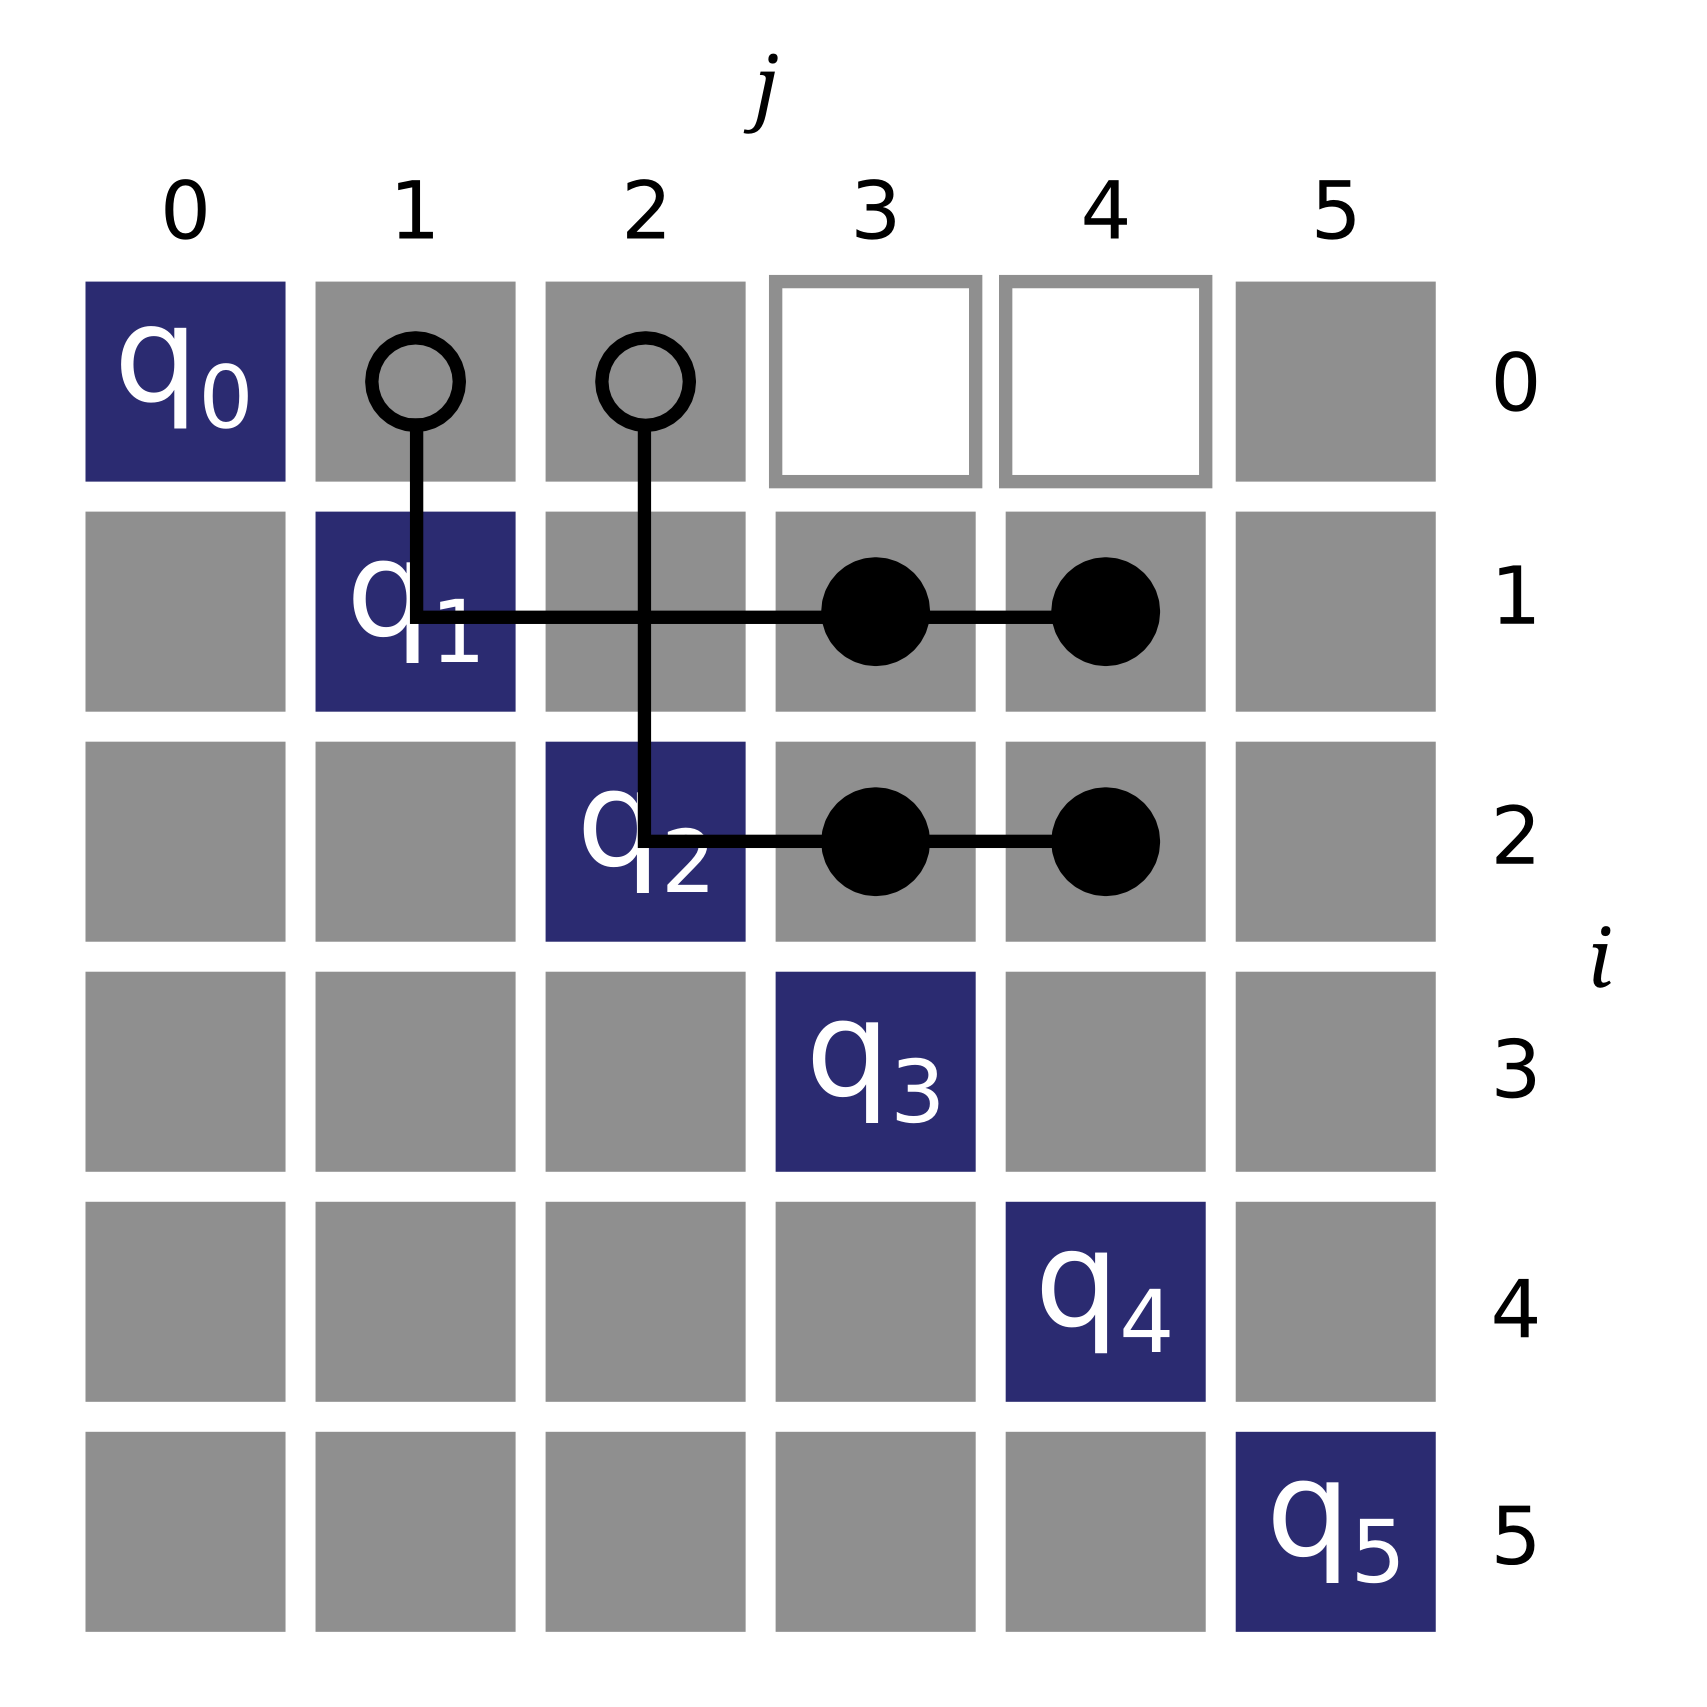
\includegraphics[width=0.33\textwidth]{img/vectorized_blocking.png}
  \caption{Vectorization of Partial Results.\label{fig:vec-blocking}}
\end{figure}

\mypar{Vectorized Blocking} Once we properly implemented blocking, it is
straight-forward to apply vectorization.
